\subsection{Прямой метод Ляпунова.}
Здесь и далее (для автономных систем) будем использовать более короткую переформулировку определений предыдущего параграфа. \\
Пусть задана автономная система $\dot{\bt{x}} = \bt{f}(\bt{x})$, где $\bt{f}: U \to \R^n$~---~гладкое векторное поле.
Для каждой точки $\bt{x}^0$ в окрестности существует и единственно решение $\bt{x} = \bt{x}(t)$ такое, что $\bt{x}(0) = \bt{x}^0$. \\
\begin{definition}
    Потоком системы будем называть отображение $\bt{g}^t(\bt{x}^0) = \bt{x}(t)$, где $\bt{x}(t)$~---~такое решение системы, что в $t = 0$ оно равно $\bt{x}^0$.
    То есть поток $\bt{g}^t$ — это отображение, которое каждой начальной точке $\bt{x}^0$ сопоставляет точку $\bt{x}^t$, в которую приходит решение в момент времени $t$. По сути, поток динамической системы -- просто сдвиг на время $t$ вдоль интегральных кривых.
\end{definition}

Нетрудно заметить, что (в пределах области определения) поток имеет групповые свойства: $\bt{g}^0 = \id, \bt{g}^{t + s} = \bt{g}^t \circ \bt{g}^s$ и $(\bt{g}^{t})^{-1} = \bt{g}^{-t}$.
\begin{note}[прим. техающего]
    Поток динамической системы не обязательно образует группу: для этого все решения должны быть определены $\forall t \in \R$.
    Подобные объекты называются <<псевдогруппами>>.
\end{note}
\begin{definition}
    Тогда определение устойчивости по Ляпунову положения равновесия $\bt{x} = 0$ автономной системы $\bt{f}$ переписывается как
    \[
        \forall \epsilon > 0 \ \exists \delta > 0: \forall \bt{x}^0 \in B_{\delta}(0) \Ra \forall t > t_0 \ \bt{g}^t(\bt{x}^0) \in B_{\epsilon}(0),
    \]
    причём $\exists \delta_0 > 0 \  \exists t_0 \  \forall \bt{x}^0 \in B_{\delta_0}(0) \   \forall t > t^0 \hookrightarrow \exists  \bt{g}^t(\bt{x}^0)$ (то есть, начиная с какого-то момента, всякий фазовый поток продолжим вправо).
\end{definition}
\begin{definition}
    Нулевое положение равновесия будем называть асимптотически устойчивым, если выполнены следующие два условия:
    \begin{itemize}
        \item Положение равновесия $\bt{x} = 0$ устойчиво по Ляпунову.
        \item $\exists \sigma > 0$ такое, что $\forall \bt{x}^0 \in B_\sigma(0) \  \exists \lim\limits_{t \ra +\infty} \bt{g}^t(\bt{x}^0) = \bt{0}$.
    \end{itemize}
\end{definition}
\begin{note}
    Определение асимптотической устойчивости положения равновесия очевидным образом распространяется на неавтономные системы.
\end{note}
\begin{theorem}[Ляпунова об устойчивости]
    Пусть для данной автономной системы существует такая гладкая функция $V: B_\rho(0) \to \R$ что выполнены следующие условия:
    \begin{itemize}
        \item[1.] $V(\bt{0}) = 0$ и $\forall \bt{x} \in B_{\rho}(0) \hookrightarrow V(\bt{x}) > 0$.
        \item[2.] Производная в силу системы (также известная как производная вдоль векторного поля $\bt{f}$ или производная Ли), определяемая как
        \[
            \dot{V} =\biggr\langle \dfrac{\partial V}{\partial \bt{x}}, \dot{\bt{x}} \biggr\rangle =  \biggr\langle \dfrac{\partial V}{\partial \bt{x}}, \bt{f} \biggr\rangle = \sum\limits_{i = 1}^n f_i \cdot \dfrac{\partial V}{\partial x_i}.
        \]
        неположительна в шаре $B_{\rho}(0)$.
    \end{itemize}
    Тогда нулевое положение равновесия устойчиво по Ляпунову.
\end{theorem}

\begin{proof}
    Из непрерывности $V$ следует что для каждого $\epsilon \in (0, \rho)$ функция $V$ достигает своего минимума на сфере $\|\bt{x}\| = \epsilon$ (причём этот минимум строго больше 0, поскольку функция $V$ положительна везде кроме $\bt{0}$).
    Обозначим его как $\sigma = \min\limits_{\|\bt{x}\| = \epsilon} V(\bt{x})$.
    Теперь рассмотрим множество $\Sigma = V^{-1}(\{\sigma\}) \cap \overline{B}_\epsilon(0)$.
    Поскольку оно ограничено и замкнуто, то оно компактно и в силу непрерывности нормы она достигает своего минимума на $\Sigma$.
    Возьмём теперь в качестве $\delta = \dfrac{1}{2}\min\limits_{\bt{x} \in \Sigma} \|\bt{x}\|$. \\
    Пусть $\bt{x}^{0} \in B_\delta(0)$.
    Поскольку $\forall t > 0 \hookrightarrow V(\bt{g}^t(\bt{x}^0)) \leq V(\bt{x}^0)$ (а это следует из условия на неположительность производной в силу системы) и по выбору $\delta$ выполняется $V(\bt{x}^0) < \sigma$, то решение $\bt{g}^t(\bt{x}^0)$ не может пересечь сферу $\|\bt{x}\| = \epsilon$ и теорема доказана.
    \begin{figure}[h!]
        \begin{center}
            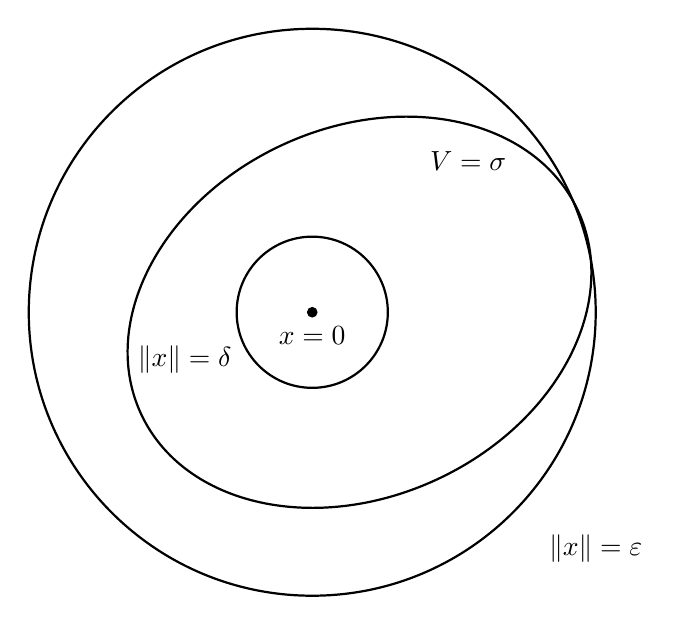
\begin{tikzpicture}[scale=6]

                \filldraw[black] (0,0) circle (0.01);
                \node at (0,-0.05) {$\bt{x}=0$};

                \draw[thick] (0,0) circle (0.16);
                \node at (-0.27,-0.1) {$\|\bt{x}\| = \delta$};

                \draw[thick] (0,0) circle (0.6);
                \node at (0.6,-0.5) {$\|\bt{x}\| = \varepsilon$};

                \draw[thick, rotate around={25:(0.1,0)}] (0.1,0) ellipse (0.51 and 0.39);
                \node at (0.33,0.32) {$V = \sigma$};

            \end{tikzpicture}
        \end{center}
        \caption{Иллюстрация к доказательству.}
    \end{figure}
\end{proof}
\begin{note}
    Функция, удовлетворяющая условиям теоремы Ляпунова об устойчивости, называется <<функция Ляпунова>>.
\end{note}
\begin{example}
    Пусть есть волчок Эйлера такой, что $C$~---~или наименьший, или наибольший момент.
    Тогда перманентные вращения $p = q = 0$ и $r = w$~---~устойчивы, и устойчивость получается при помощи функции Ляпунова
    \[
        V_{\pm} = \dfrac{T^2}{w^2} \pm (K^2 - CT).
    \]
\end{example}
\begin{theorem}[Барбашина-Красовского, об асимптотической устойчивости]
    Пусть для автономной системы $\bt{f}$ существует функция $V$, для которой выполнены условия теоремы Ляпунова об устойчивости (то есть условия $1.$ и $2.$ предыдущей теоремы).
    Пусть выполнено следующее условие:
    \begin{itemize}
        \item[3.] Множество $\Sigma = \dot{V}^{-1}(\{0\})$ не содержит <<целых>> траекторий динамической системы кроме $\bt{x} \equiv 0$.
    \end{itemize}
    Тогда положение равновесия $\bt{x} = 0$ является асимптотически устойчивым.
\end{theorem}
\begin{proof}
    Предположим, что $0$~---~асимптотически неустойчивое равновесие.
    Оно уже устойчиво по теореме Ляпунова, но
    \[
        \forall \sigma > 0 \  \exists \bt{x}^0 \in B_{\sigma}(0) \hookrightarrow \nexists \lim\limits_{t \ra +\infty} \bt{g}^t(\bt{x}^0) \vee \lim\limits_{t \ra +\infty} \bt{g}^{t}(\bt{x}^0) \neq 0.
    \]
    Заметим, что предел $V \circ \bt{g}^{t}(\bt{x}^0), t \ra +\infty$ всегда существует (из монотонности композиции).
    Пусть он равен $V_\infty > 0$ (если он равен нулю -- то решение сходится к $\bt{0}$, что не так по предположению).
    С другой стороны, $\dot{V} \circ \bt{g}^t(\bt{x}^0) \ra 0, t \ra +\infty$.
    Поскольку множество предельных точек $\bt{g}^t(\bt{x}^0)$~---~компактно и остаётся на месте под действием фазового потока, то оно должно состоять ровно из одной точки -- $\bt{0}$, по третьему условию.
    Значит мы приходим к противоречию и получаем асимптотическую устойчивость нулевого положения равновесия.
\end{proof}
\begin{note}
    Множество предельных точек $\bt{g}^t(\bt{x}^0)$ -- замкнуто по определению: оно состоит из предельных точек всевозможных последовательностей $t_n$ таких, что $t_n \ra +\infty, n \ra \infty$.
    И оно ограничено, поскольку положение равновесия устойчиво по Ляпунову -- а следовательно траектории не уходят на бесконечность.
    Замкнутое и ограниченное множество в евклидовом пространстве компактно.
\end{note}
\begin{note}
    Предел $\dot{V}(\bt{g}^t(\bt{x}^0))$ в бесконечности существует и равен нулю из сходимости $V(\bt{g}^t(\bt{x}^0))$ к некоторой точке $V_\infty$.
\end{note}
\begin{theorem}[Четаева, о неустойчивости]
    Пусть существует гладкая функция $V: B_{\rho}(0) \to \R$ такая, что
    \begin{itemize}
        \item $V(\bt{0}) = 0$ и $\bt{0} \in \partial \Omega$, где $\Omega = \{\bt{x} \in B_{\rho}(0) \mid V(\bt{x}) \neq 0\}$.
        \item $V|_{\Int \Omega} > 0$.
        \item $\dot{V}|_{\Omega} \geq 0$.
        \item В $\dot{V}^{-1}(0)$ нет целых траекторий решений системы кроме $\bt{x} = 0$.
    \end{itemize}
    Тогда нулевое равновесие неустойчиво.
\end{theorem}
\begin{proof}
    Предположим, что равновесие устойчиво.
    Тогда $\exists \delta > 0$ такое, что $\forall \bt{x}^0 \in B_{\rho}(0)$ выполняется $\forall t \geq 0 \ \bt{g}^t(\bt{x}^0) \in B_{\delta}(0)$.
    Пусть $\bt{x} \in B_\delta(0) \cap \Omega$ и $V(\bt{x}) \neq 0$.
    Из условий теоремы следует, что $\forall t \geq 0 \hookrightarrow V \circ \bt{g}^t(\bt{x}) \geq V(\bt{x}) > 0$.
    Тогда, аналогично предыдущей теореме, у нас существуют пределы $\dot{V}$ и $V \circ \bt{g}^t(\bt{x})$ и множество предельных точек будет содержать иные решения кроме нулевого.
\end{proof}
\begin{note}
    Последние два условия теоремы можно заменить на $\dot{V}|_{\Omega} > 0$.
\end{note}
\begin{note}[прим. техающего]
    Любое решение, начинающееся в $\Omega$, покинет шар $B_\rho(0)$.
\end{note}
\begin{note}
    В некоторых источников функция, удовлетворяющая условиям теоремы Четаева называется <<функцией Четаева>>.
\end{note}
\begin{theorem}[Лагранжа-Дирихле, об устойчивости положения равновесия в консервативных системах]
    Для консервативной механической системы строгий минимум потенциальной энергии является достаточным условием устойчивого равновесия.
\end{theorem}
\begin{proof}
    Для доказательства теоремы достаточно взять в качестве функции Ляпунова полную энергию $E = T + \Pi$ и применить теорему Ляпунова.
\end{proof}
\begin{note}[прим. техающего]
    Теорема Лагранжа-Дирихле допускает обращение в случае аналитической функции Лагранжа:
    \begin{theorem}
        Если функция Лагранжа консервативной системы аналитическая, а положение равновесия не является изолированным локальным минимумом потенциальной энергии, то оно неустойчиво.
    \end{theorem}
\end{note}